\section{Monolayers}
\label{sec:mono}

\subsection{Execution}

The following is conducted for two different unknown TMDCs:
Firstly the scotch tape technique is used, to separate the layers from a thick crystal.
These layers are then transferred to a gel strip, from which they are subsequently transferred onto a silicon wafer that has an SiO$_2$ layer on top.

In order to now find pieces on the wafer that are monolayers, an optical microscope is used, utilizing the fact that due to the different refractive indeces of Si, the SiO$_2$ and the deposited material different thicknesses appear in different colors \cite{benameur2011}.
The samples are then transferred to a widefield microscope, a schematic of which is shown in \cref{fig_widefield}.
%TODO da noch was beschreibendes zu
The lense used has a numerical aperture of \SI{0.9}{}.
Apart from also having imaging properties, a slit can be inserted into the widefield microscope, to record a spectrum using a basic light spectrometer.
Due to the insertion of the slit, imaging properties in one direction are lost in the process.
For both microscopes a sample with a grating of known grid size is used, to get the scale for the image taken of the samples.
For one material two specimen (pieces including monolayers) are examined and for the other one only one spot is examined.

\begin{figure}[!ht]
    \centering
    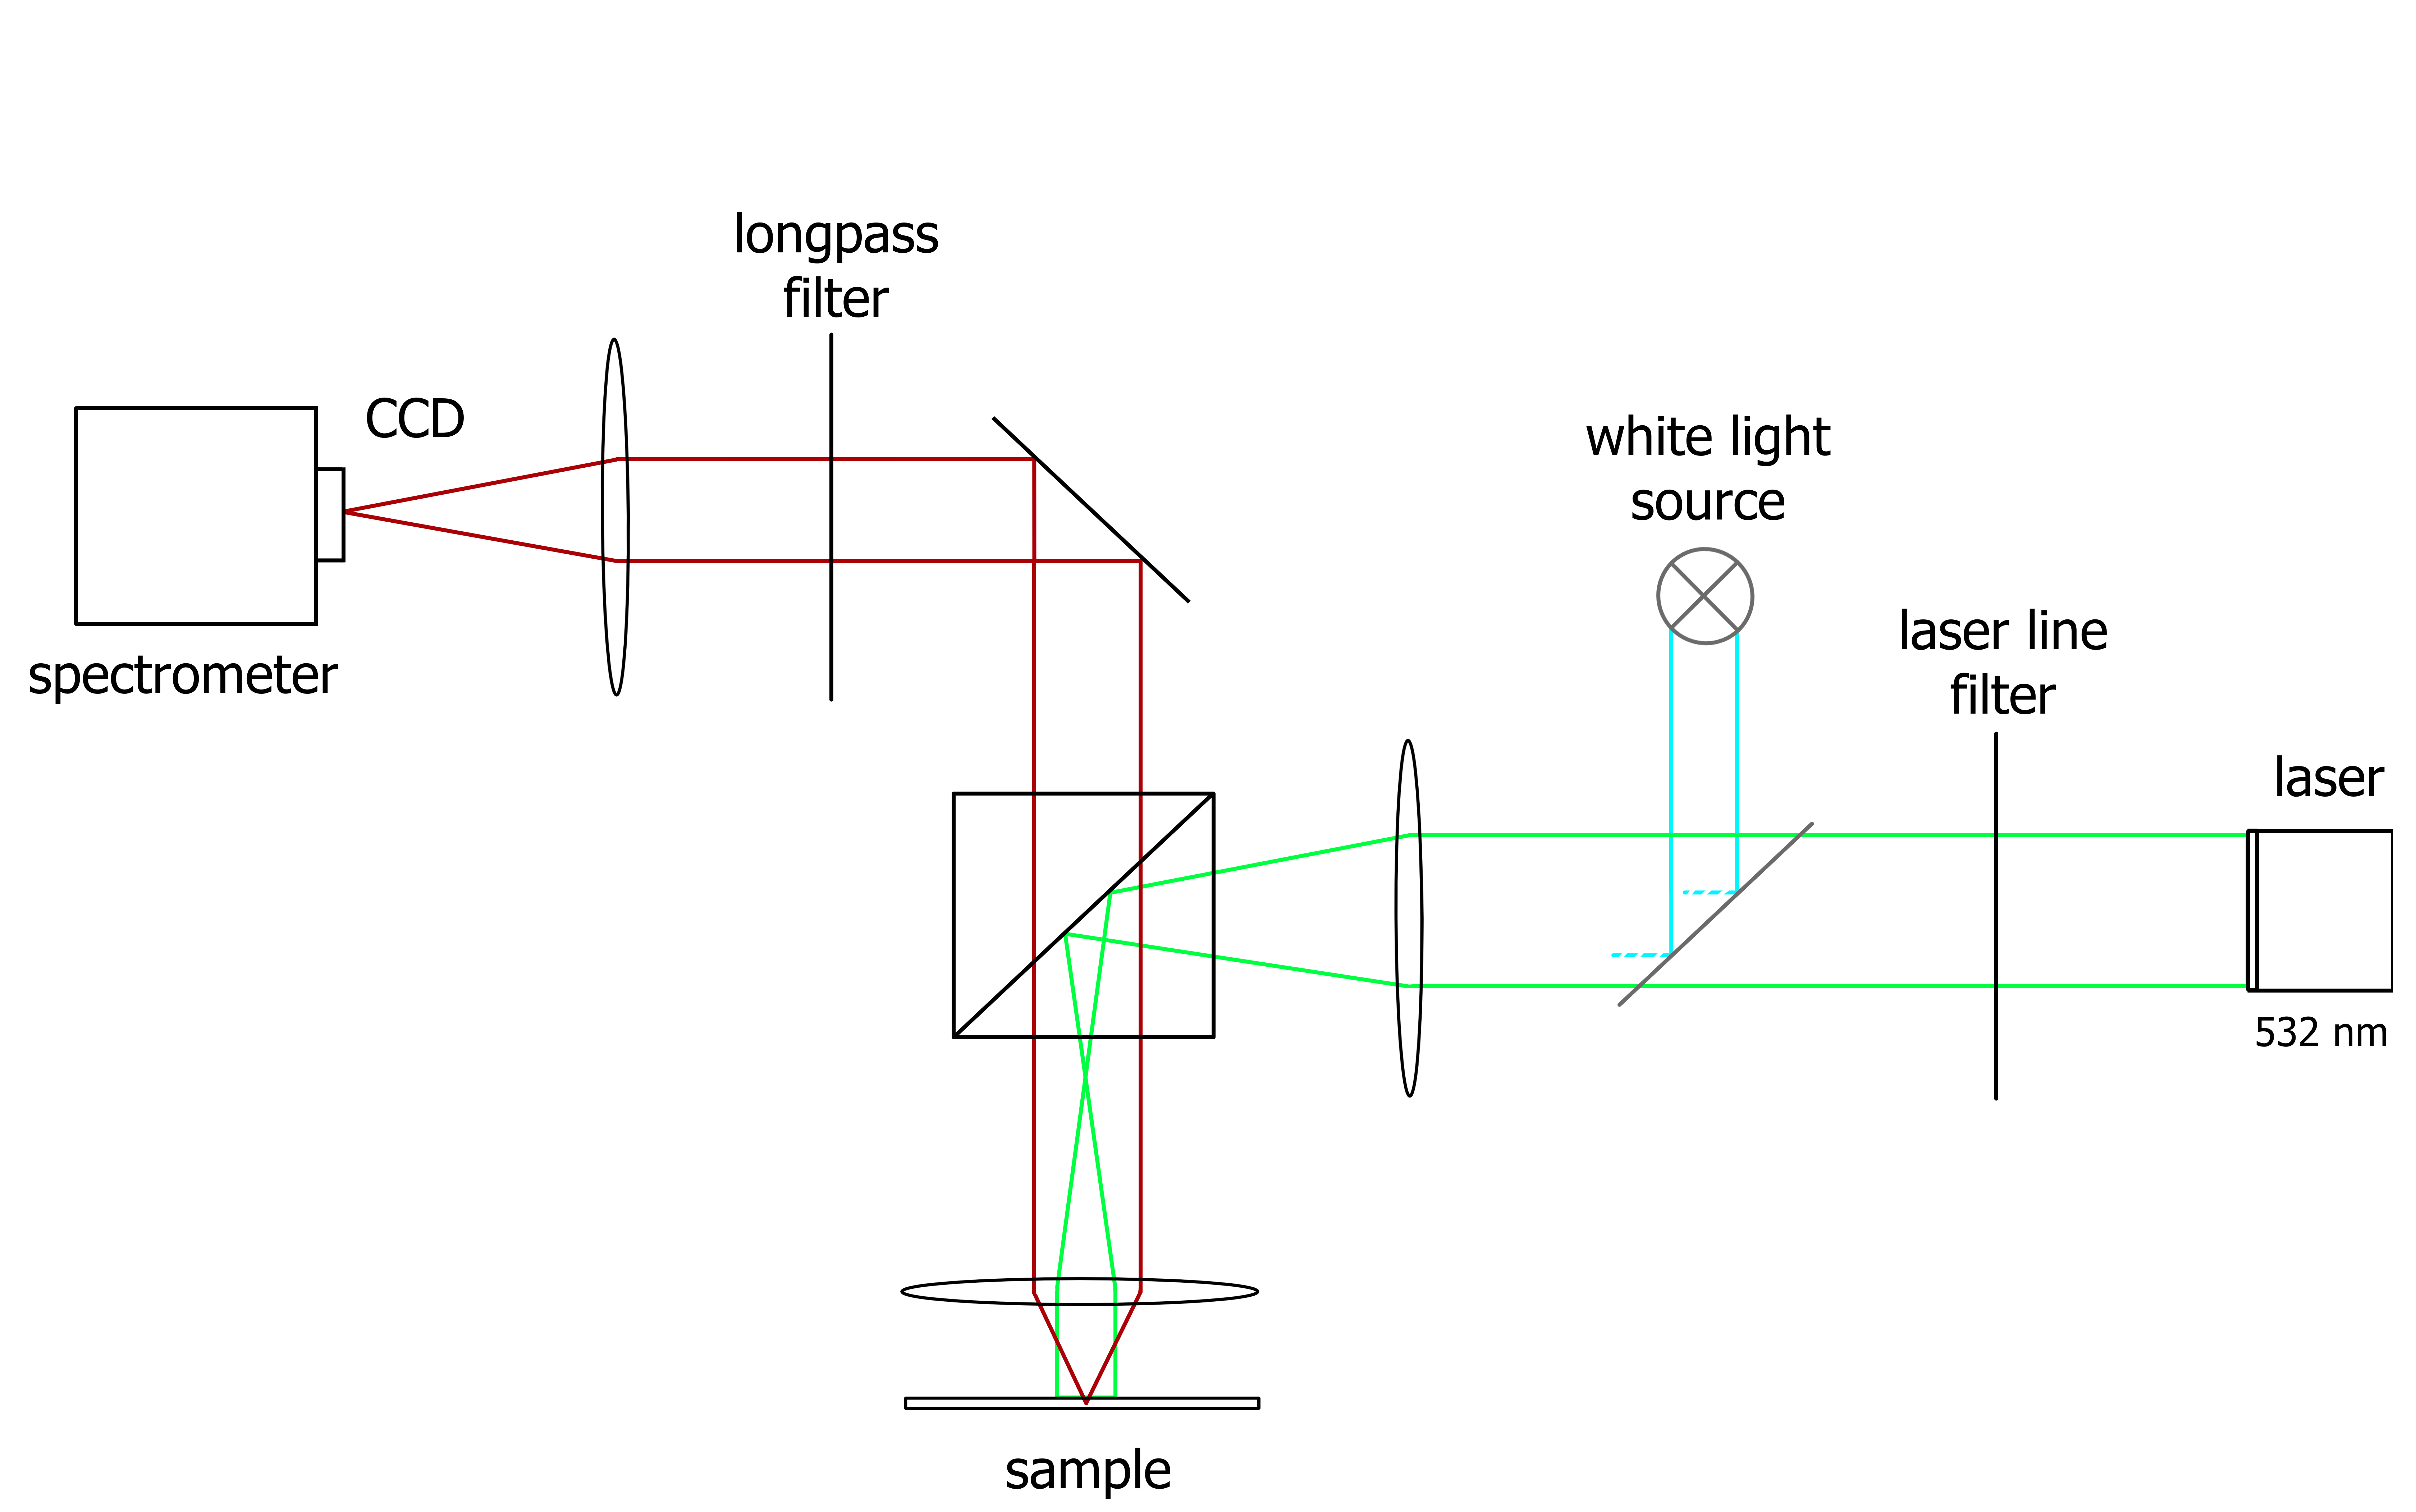
\includegraphics[width=0.7\textwidth]{img/setup1.png}
    \caption{Schematic of the widefield microscope used to record photoluminescence spectra. The detector corresponds to a spectrometer.}
    \label{fig_widefield}
\end{figure}


\subsection{Analysis}

In \crefrange{fig_mono_spec1}{fig_mono_spec3} the image recorded using the interference based and the widefield microscope are shown.
As an example for the first specimen the image containing the spectrum is shown in \cref{fig_mono_spec1_spec}.
In the interference based microscope monolayers appear as light fawn (hex color code \#A97E5C), while in the widefield microscope they appear bright white.
From these images for each specimen the spectrum is calculated by summing over multiple lines of pixels and can be seen in \cref{fig_mono_1dspectra}.

\begin{figure}[!ht]
    \centering
    \begin{subfigure}{0.47\textwidth}
        \centering
        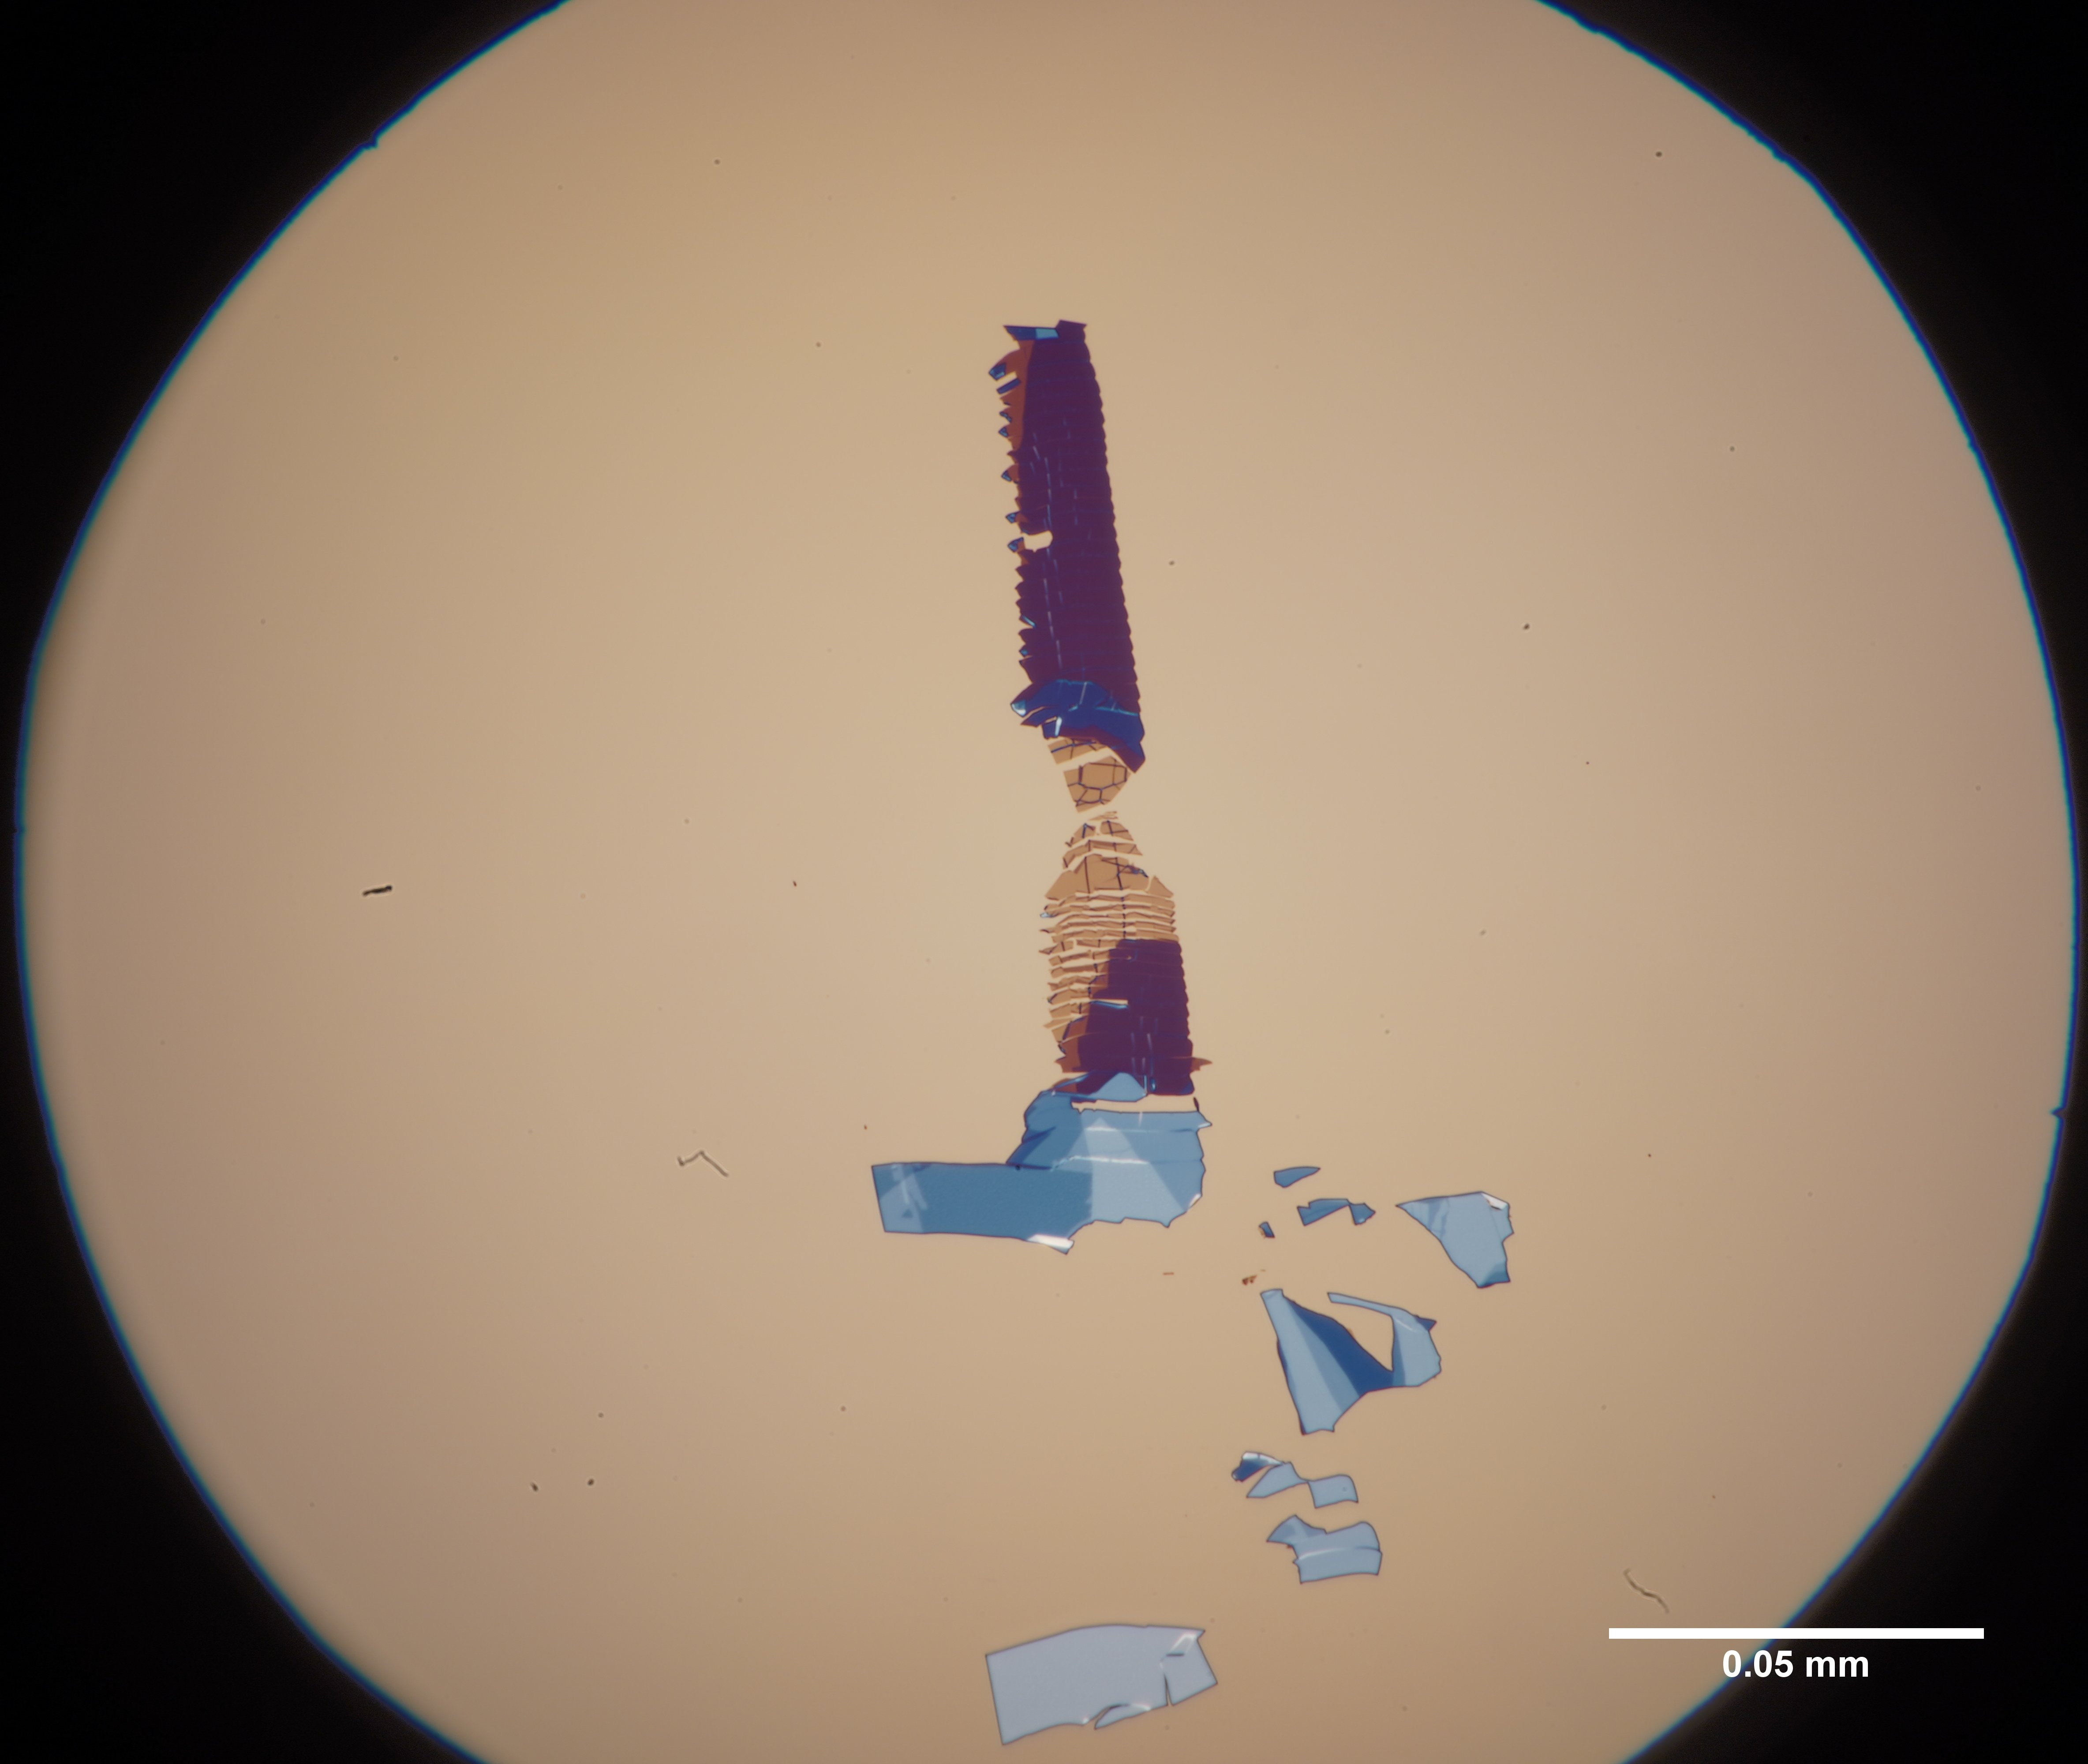
\includegraphics[width=1.0\textwidth]{img/output_t1/M1_3_100_adj}
        \caption{interference}
	      \label{fig_mono_spec1_int}
    \end{subfigure}
    \hfill
    \begin{subfigure}{0.47\textwidth}
        \centering
        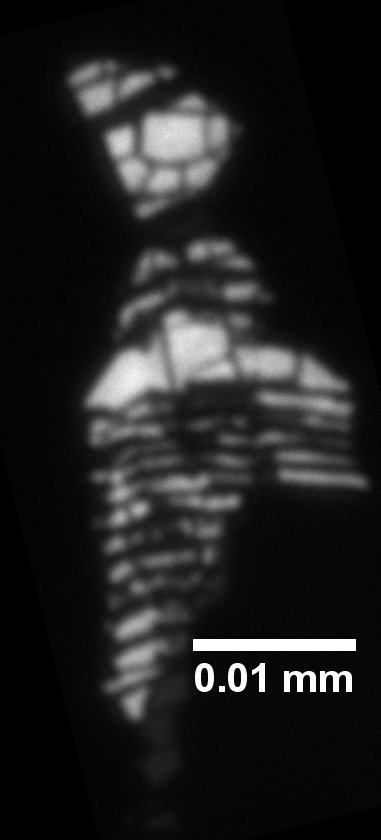
\includegraphics[width=\textwidth]{img/output_t1/M1_3_50_adj_photo}
        \caption{widefield}
	      \label{fig_mono_spec1_wide}
    \end{subfigure}
    \begin{subfigure}{0.7\textwidth}
        \centering
        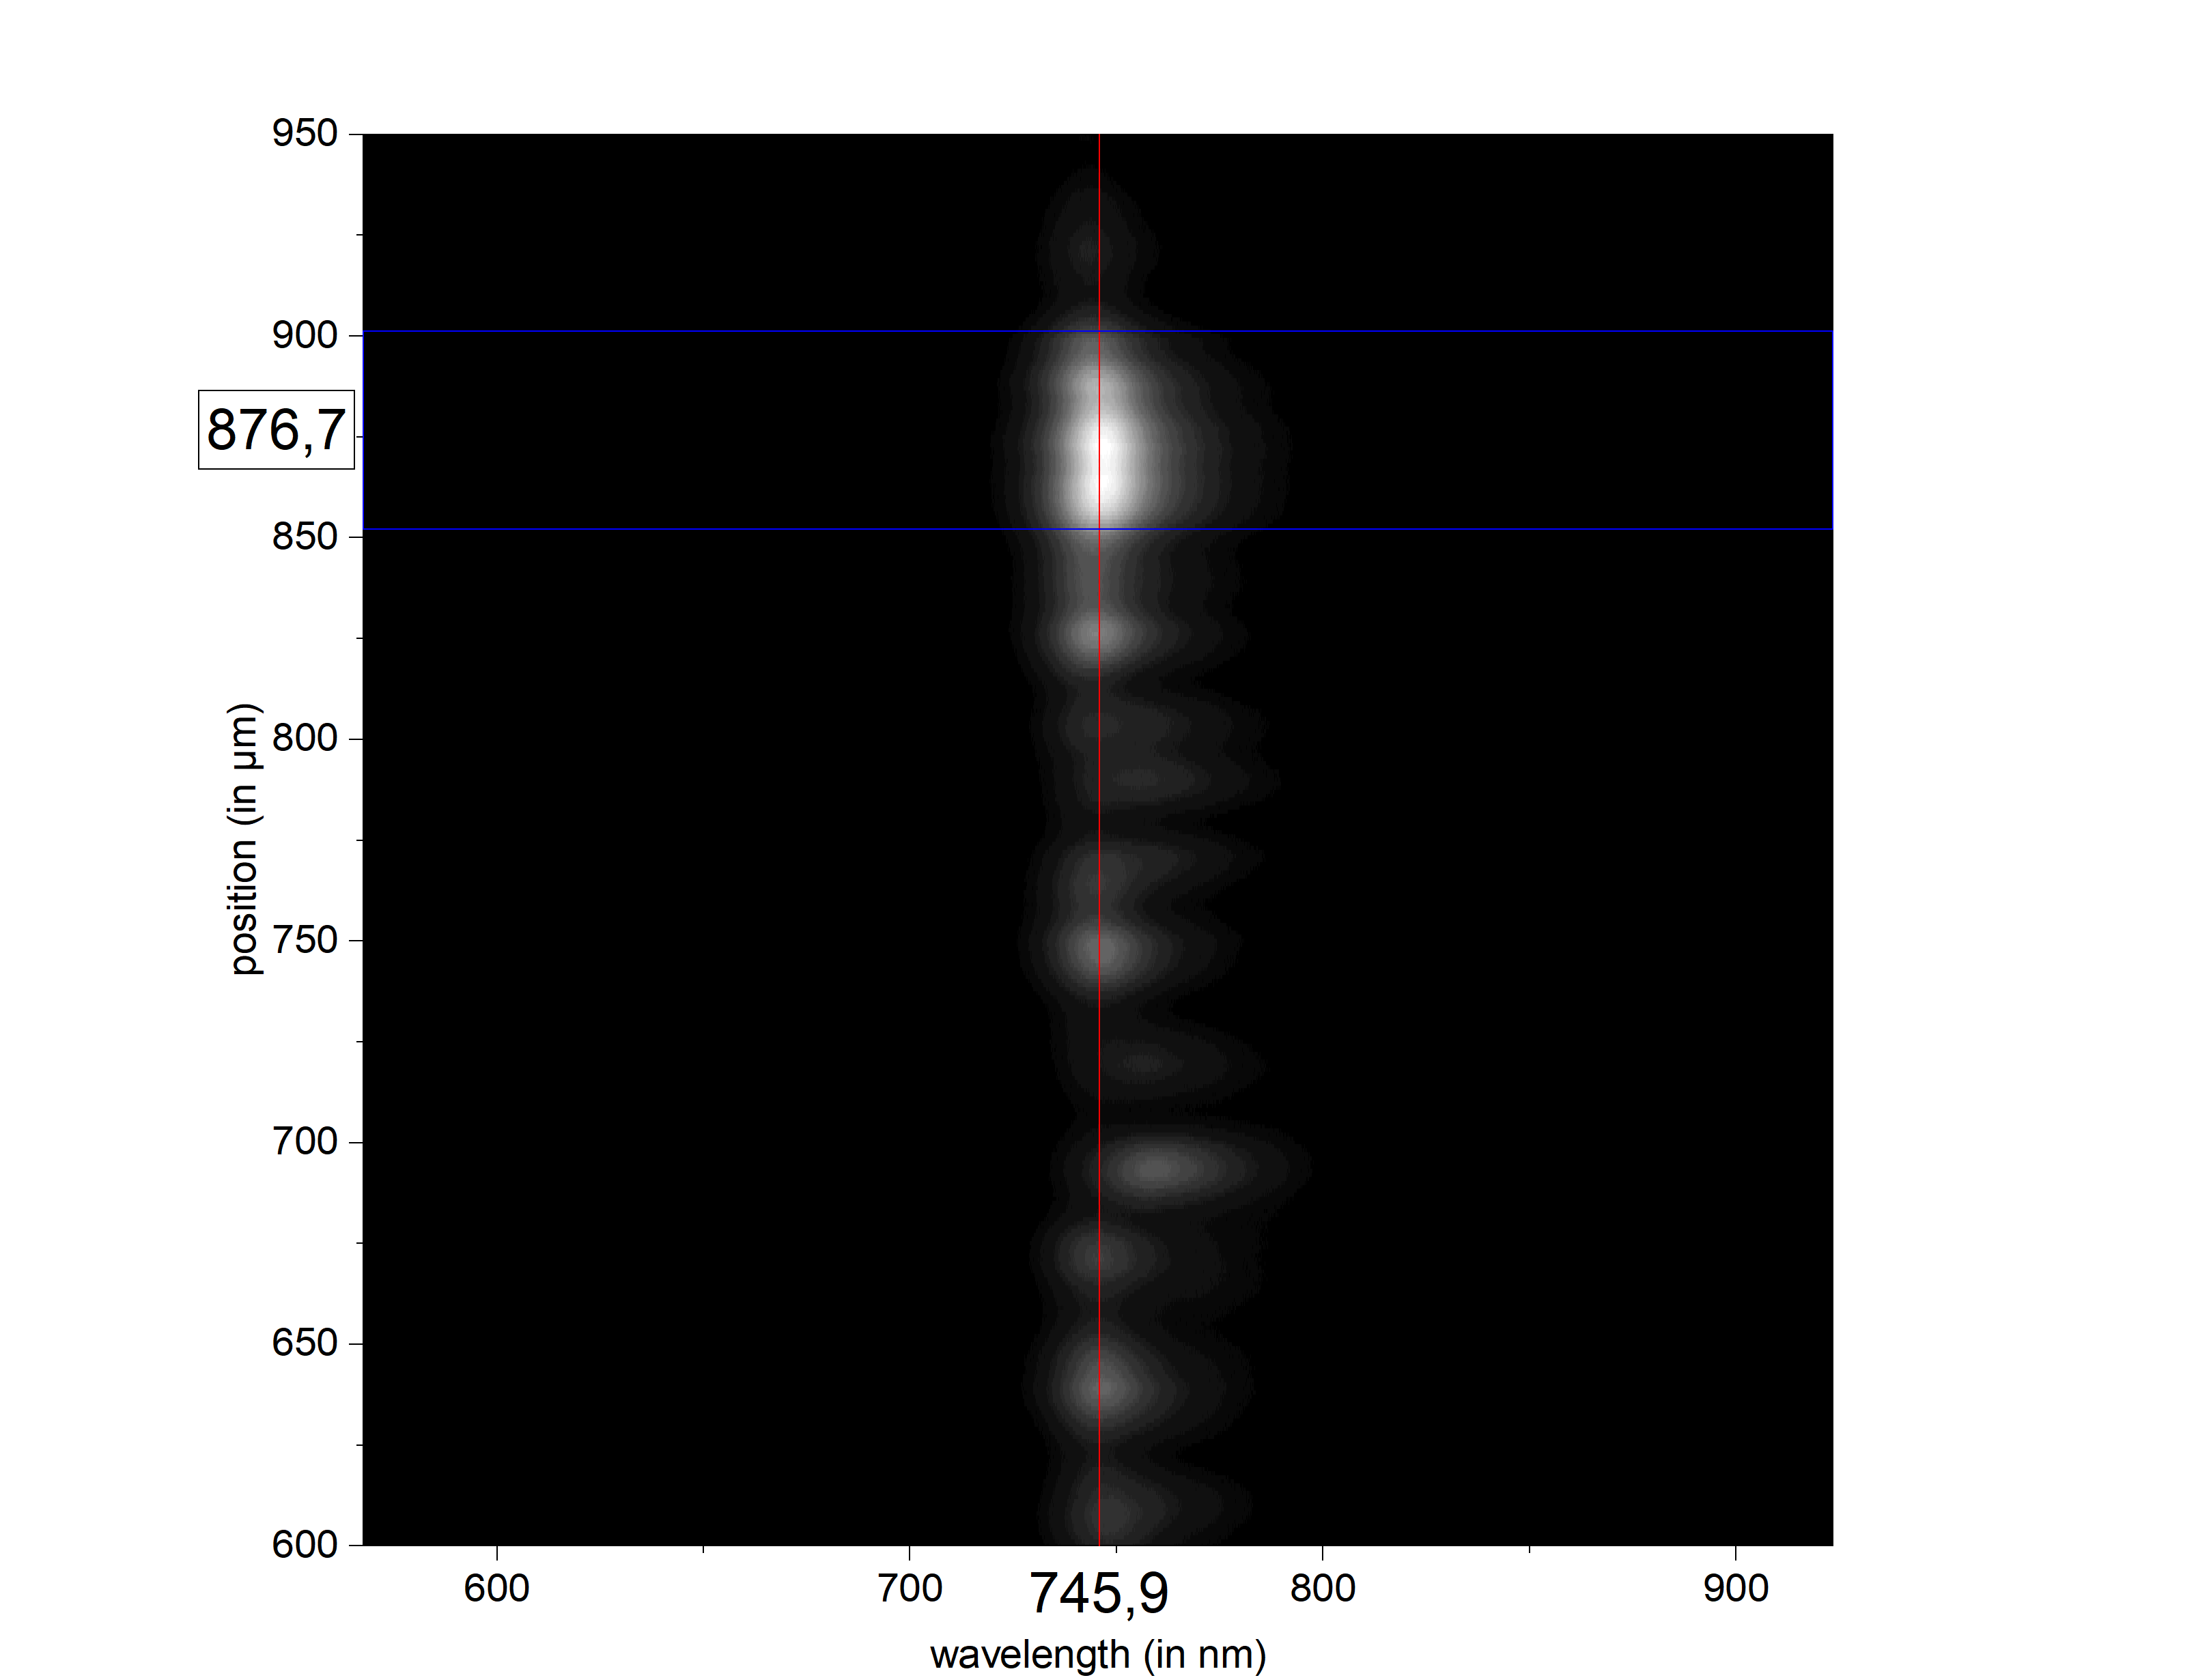
\includegraphics[width=\textwidth]{img/output_t1/bild_m1-3.png}
        \caption{spectrum}
	      \label{fig_mono_spec1_spec}
    \end{subfigure}
    \caption{Optical microscopy images for specimen 1 of material 1 gained by the interference based microscope and the widefield microscope. Additionally the image containing the spectrum in one direction is shown and the part that is used for the spectrum in \cref{fig_mono_1dspectra} lies between the blue lines.}
	\label{fig_mono_spec1} % 3->1
\end{figure}

\begin{figure}[!ht]
    \centering
    \begin{subfigure}{0.47\textwidth}
        \centering
        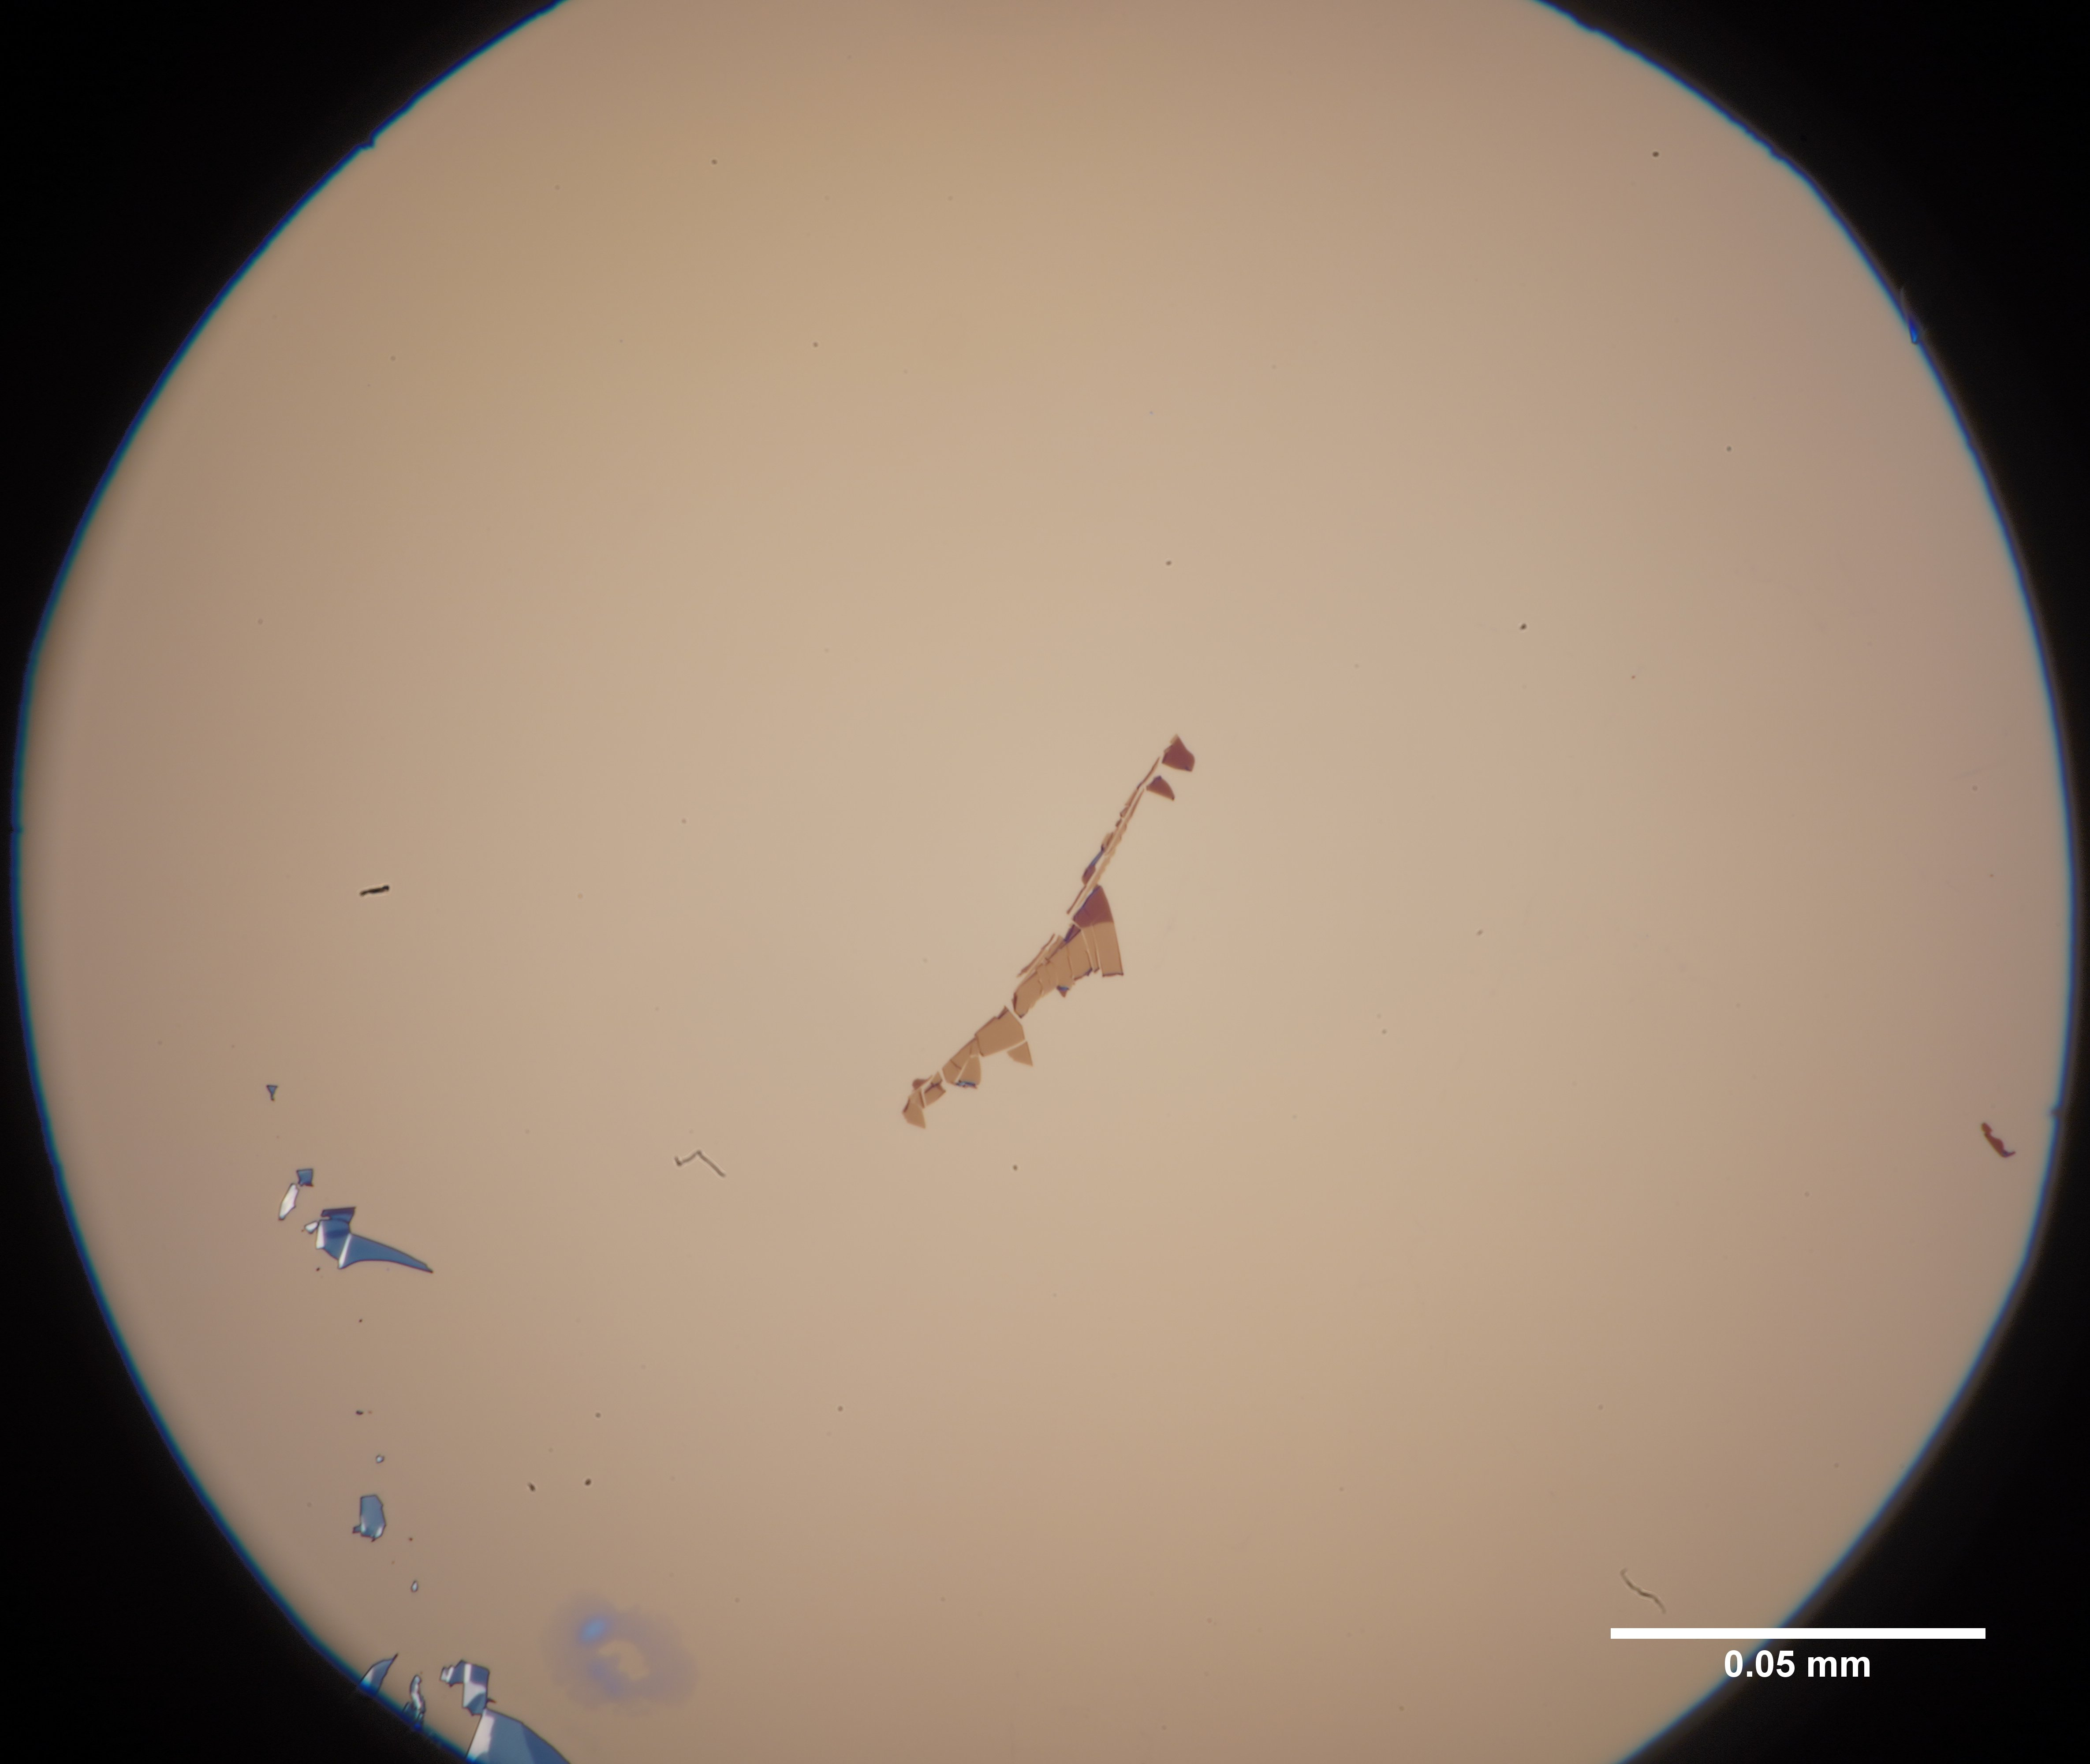
\includegraphics[width=\textwidth]{img/output_t1/M1_2_100_adj}
        \caption{interference}
	      \label{fig_mono_spec2_int}
    \end{subfigure}
    \hfill
    \begin{subfigure}{0.47\textwidth}
        \centering
        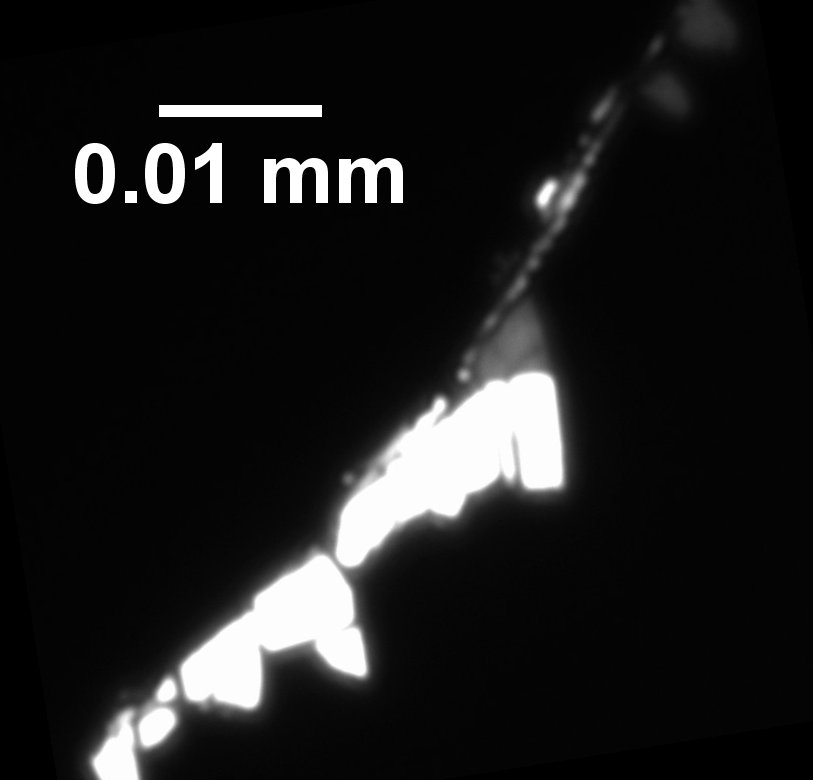
\includegraphics[width=\textwidth]{img/output_t1/M1_2_50_adj_photo}
        \caption{widefield}
	      \label{fig_mono_spec2_wide}
    \end{subfigure}
    \caption{Optical microscopy images for specimen 2 of material 1 gained by the interference based microscope and the widefield microscope.}
	\label{fig_mono_spec2} %2->2
\end{figure}

\begin{figure}[!ht]
    \centering
    \begin{subfigure}{0.47\textwidth}
        \centering
        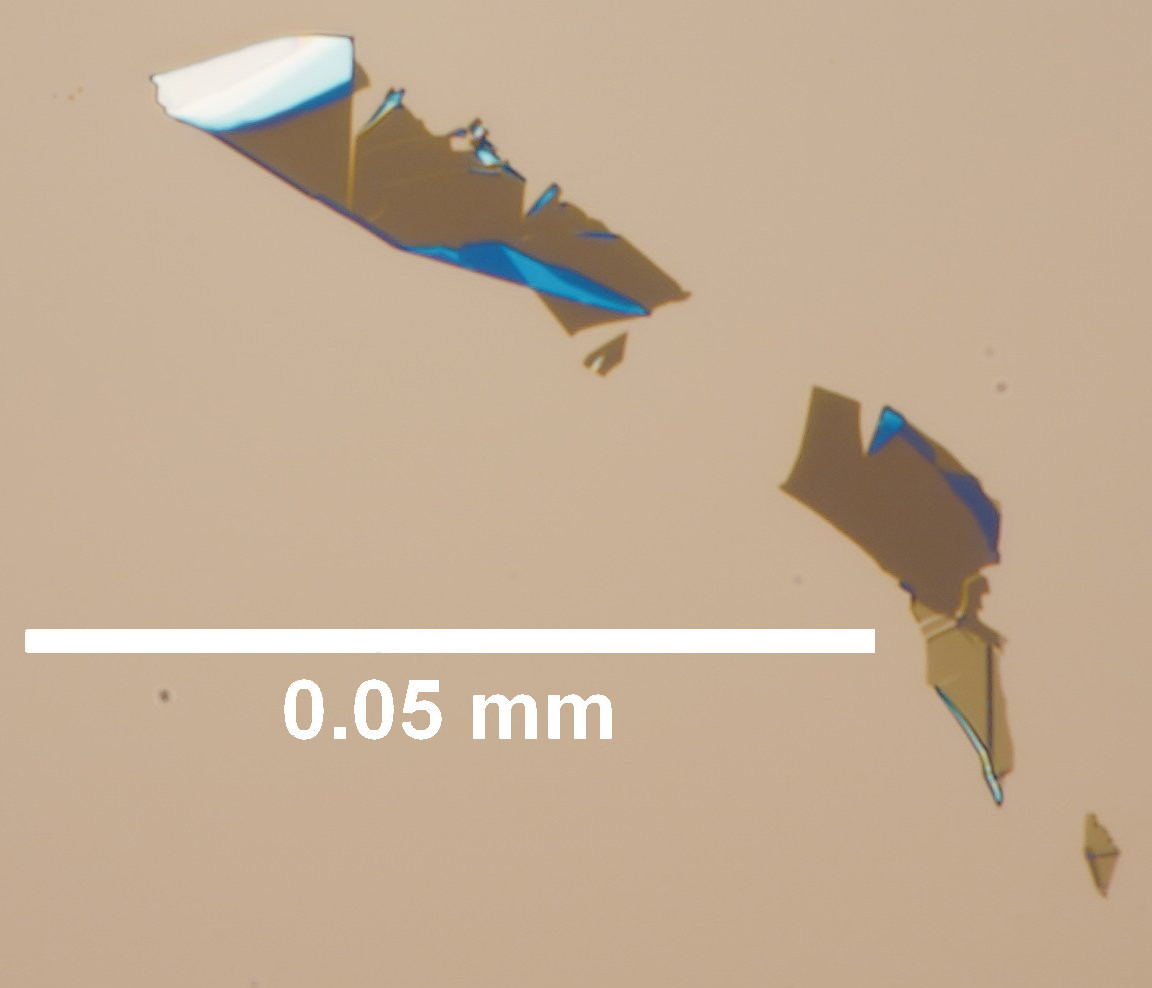
\includegraphics[width=1.0\textwidth]{img/output_t1/M2_1_100_adj}
        \caption{interference}
	      \label{fig_mono_spec3_int}
    \end{subfigure}
    \hfill
    \begin{subfigure}{0.47\textwidth}
        \centering
        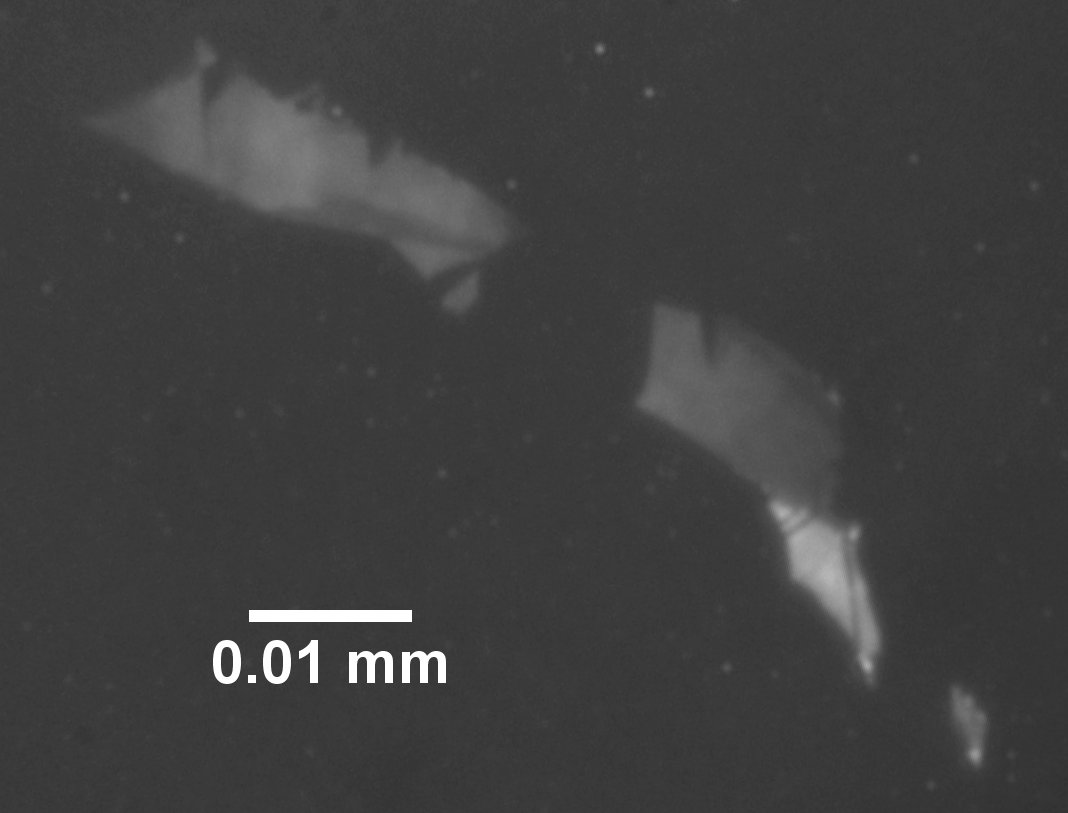
\includegraphics[width=\textwidth]{img/output_t1/M2_1_50_adj_photo4}
        \caption{widefield}
	      \label{fig_mono_spec3_wide}
    \end{subfigure}
    \caption{Optical microscopy images for material 2 gained by the interference based microscope and the widefield microscope.}
	\label{fig_mono_spec3} %mat2 -> 3
\end{figure}

\begin{figure}[!ht]
    \centering
    \begin{subfigure}{0.7\textwidth}
        \centering
        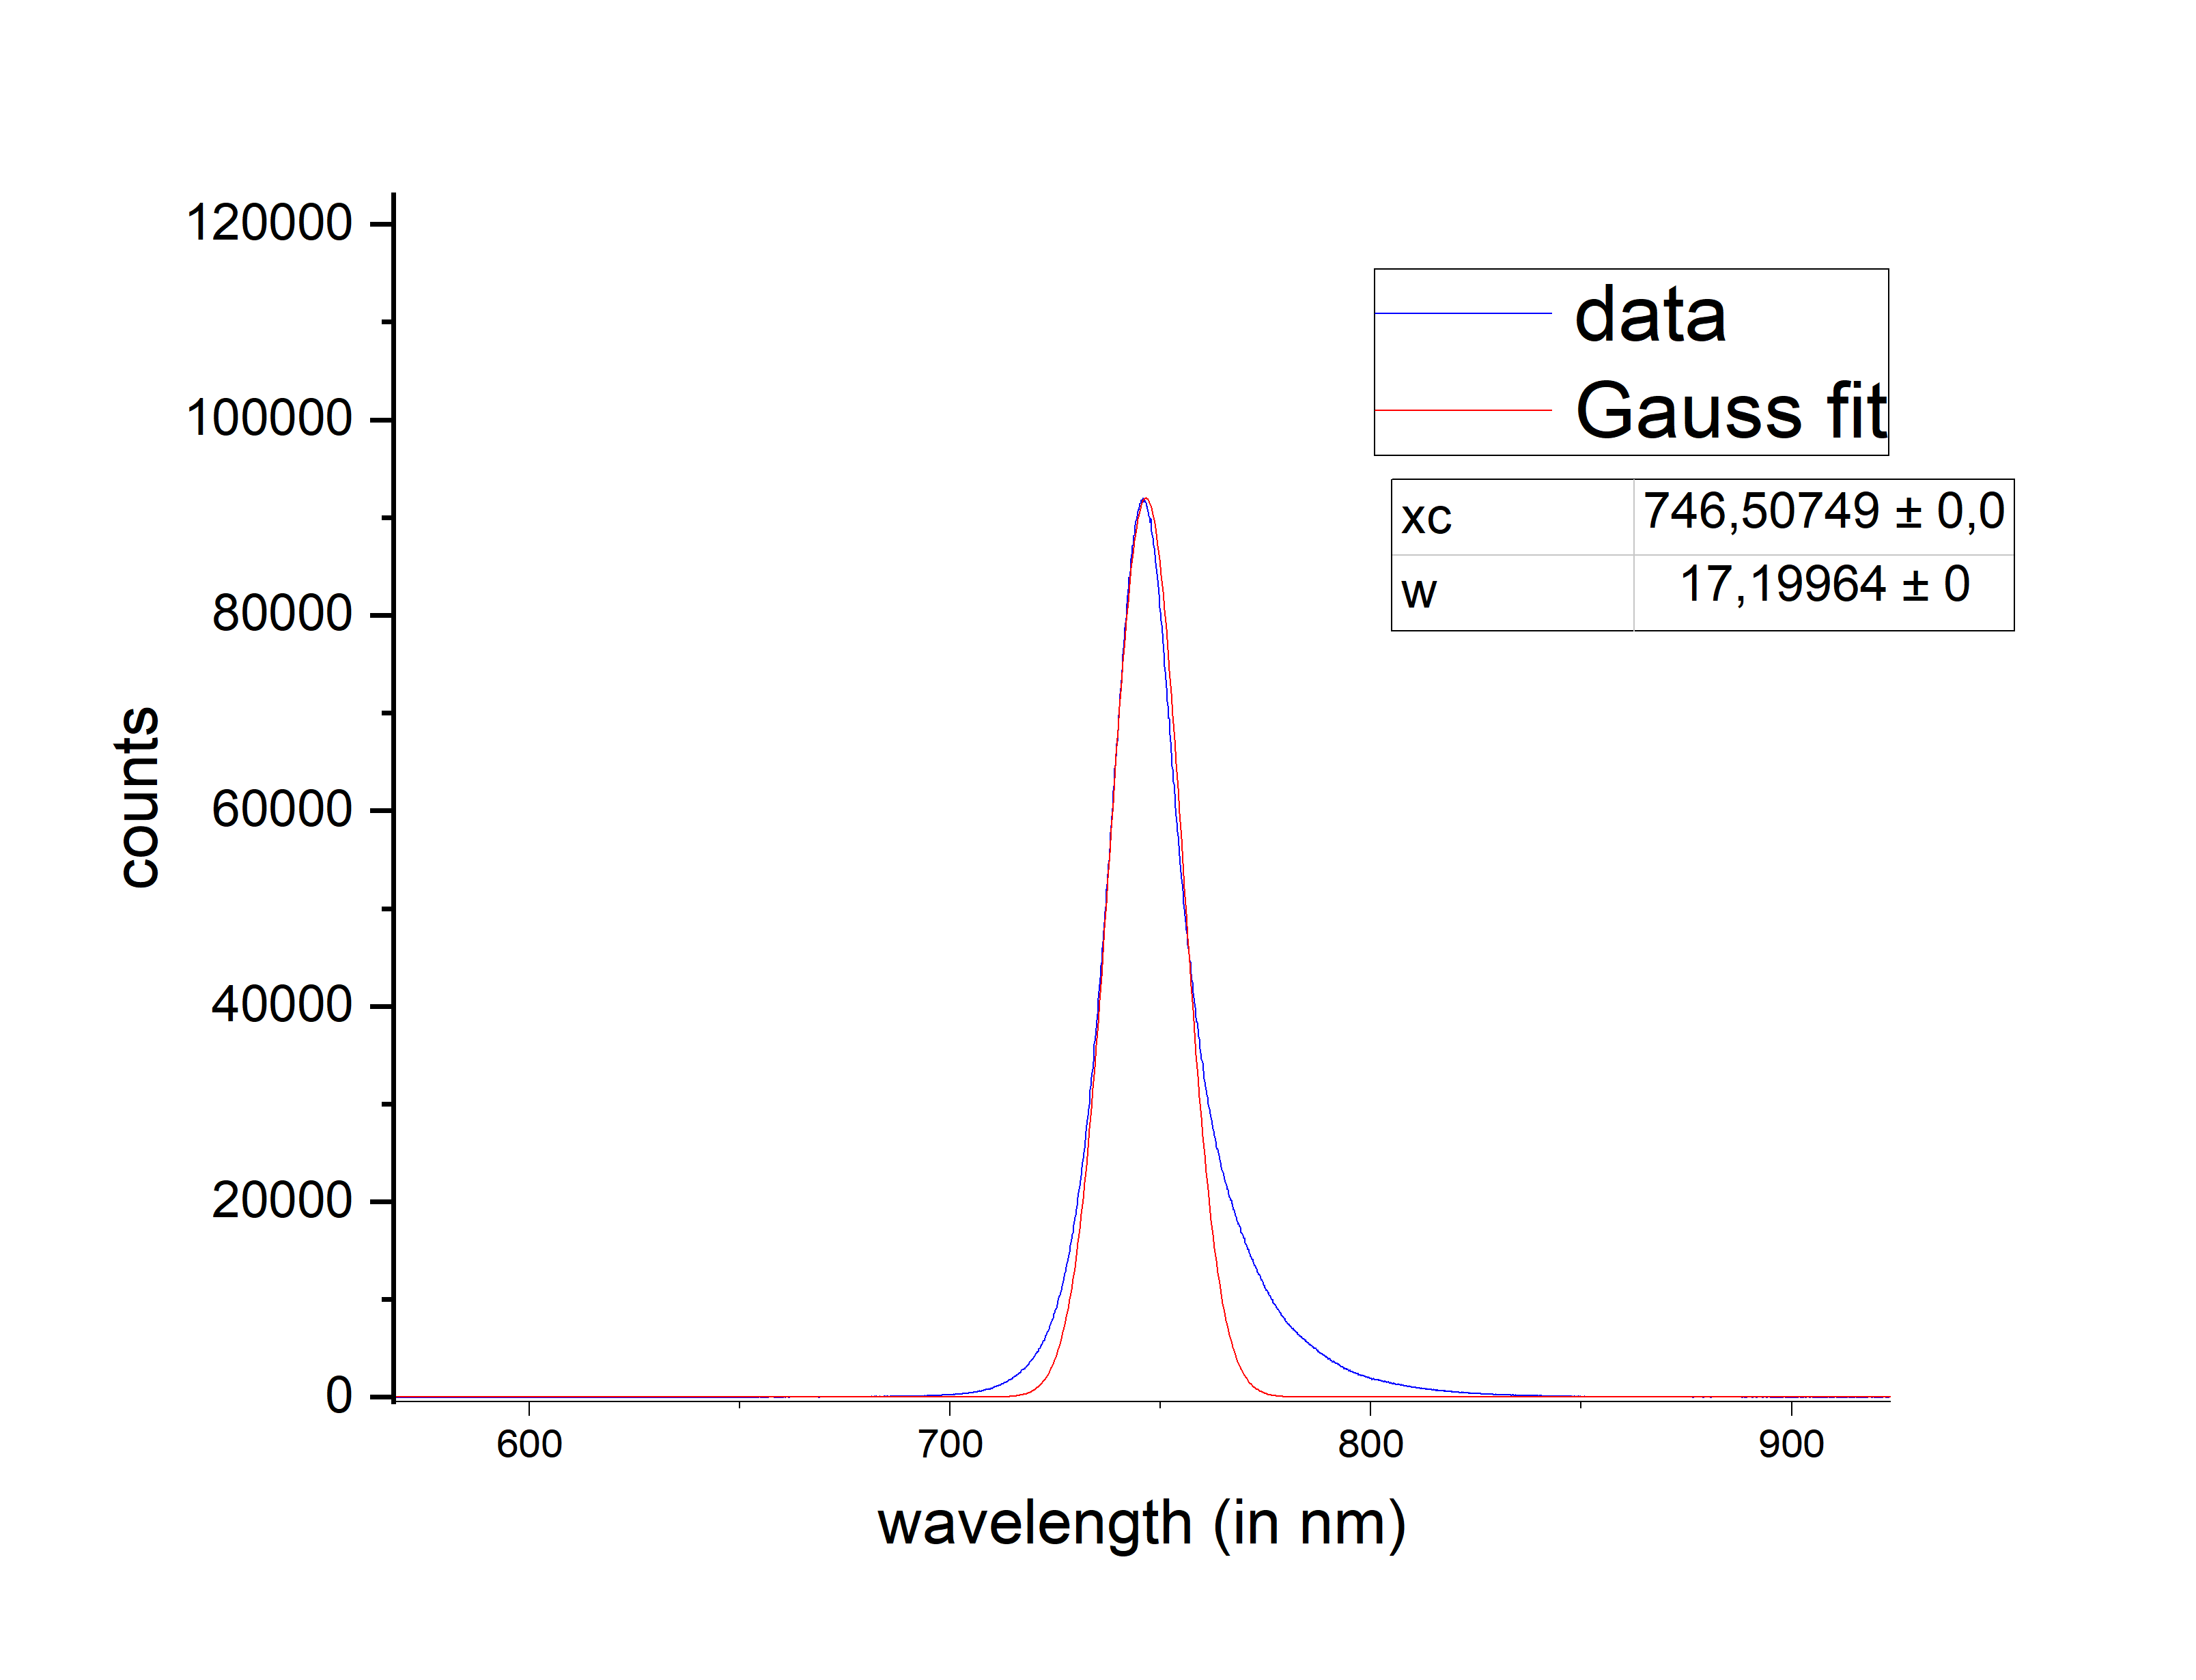
\includegraphics[width=1.0\textwidth]{img/output_t1/spekt_m1-3}
        \caption{mat. 1, spec. 1}
	      \label{fig_mono_spec1_1dspec}
    \end{subfigure}
    \begin{subfigure}{0.7\textwidth}
        \centering
        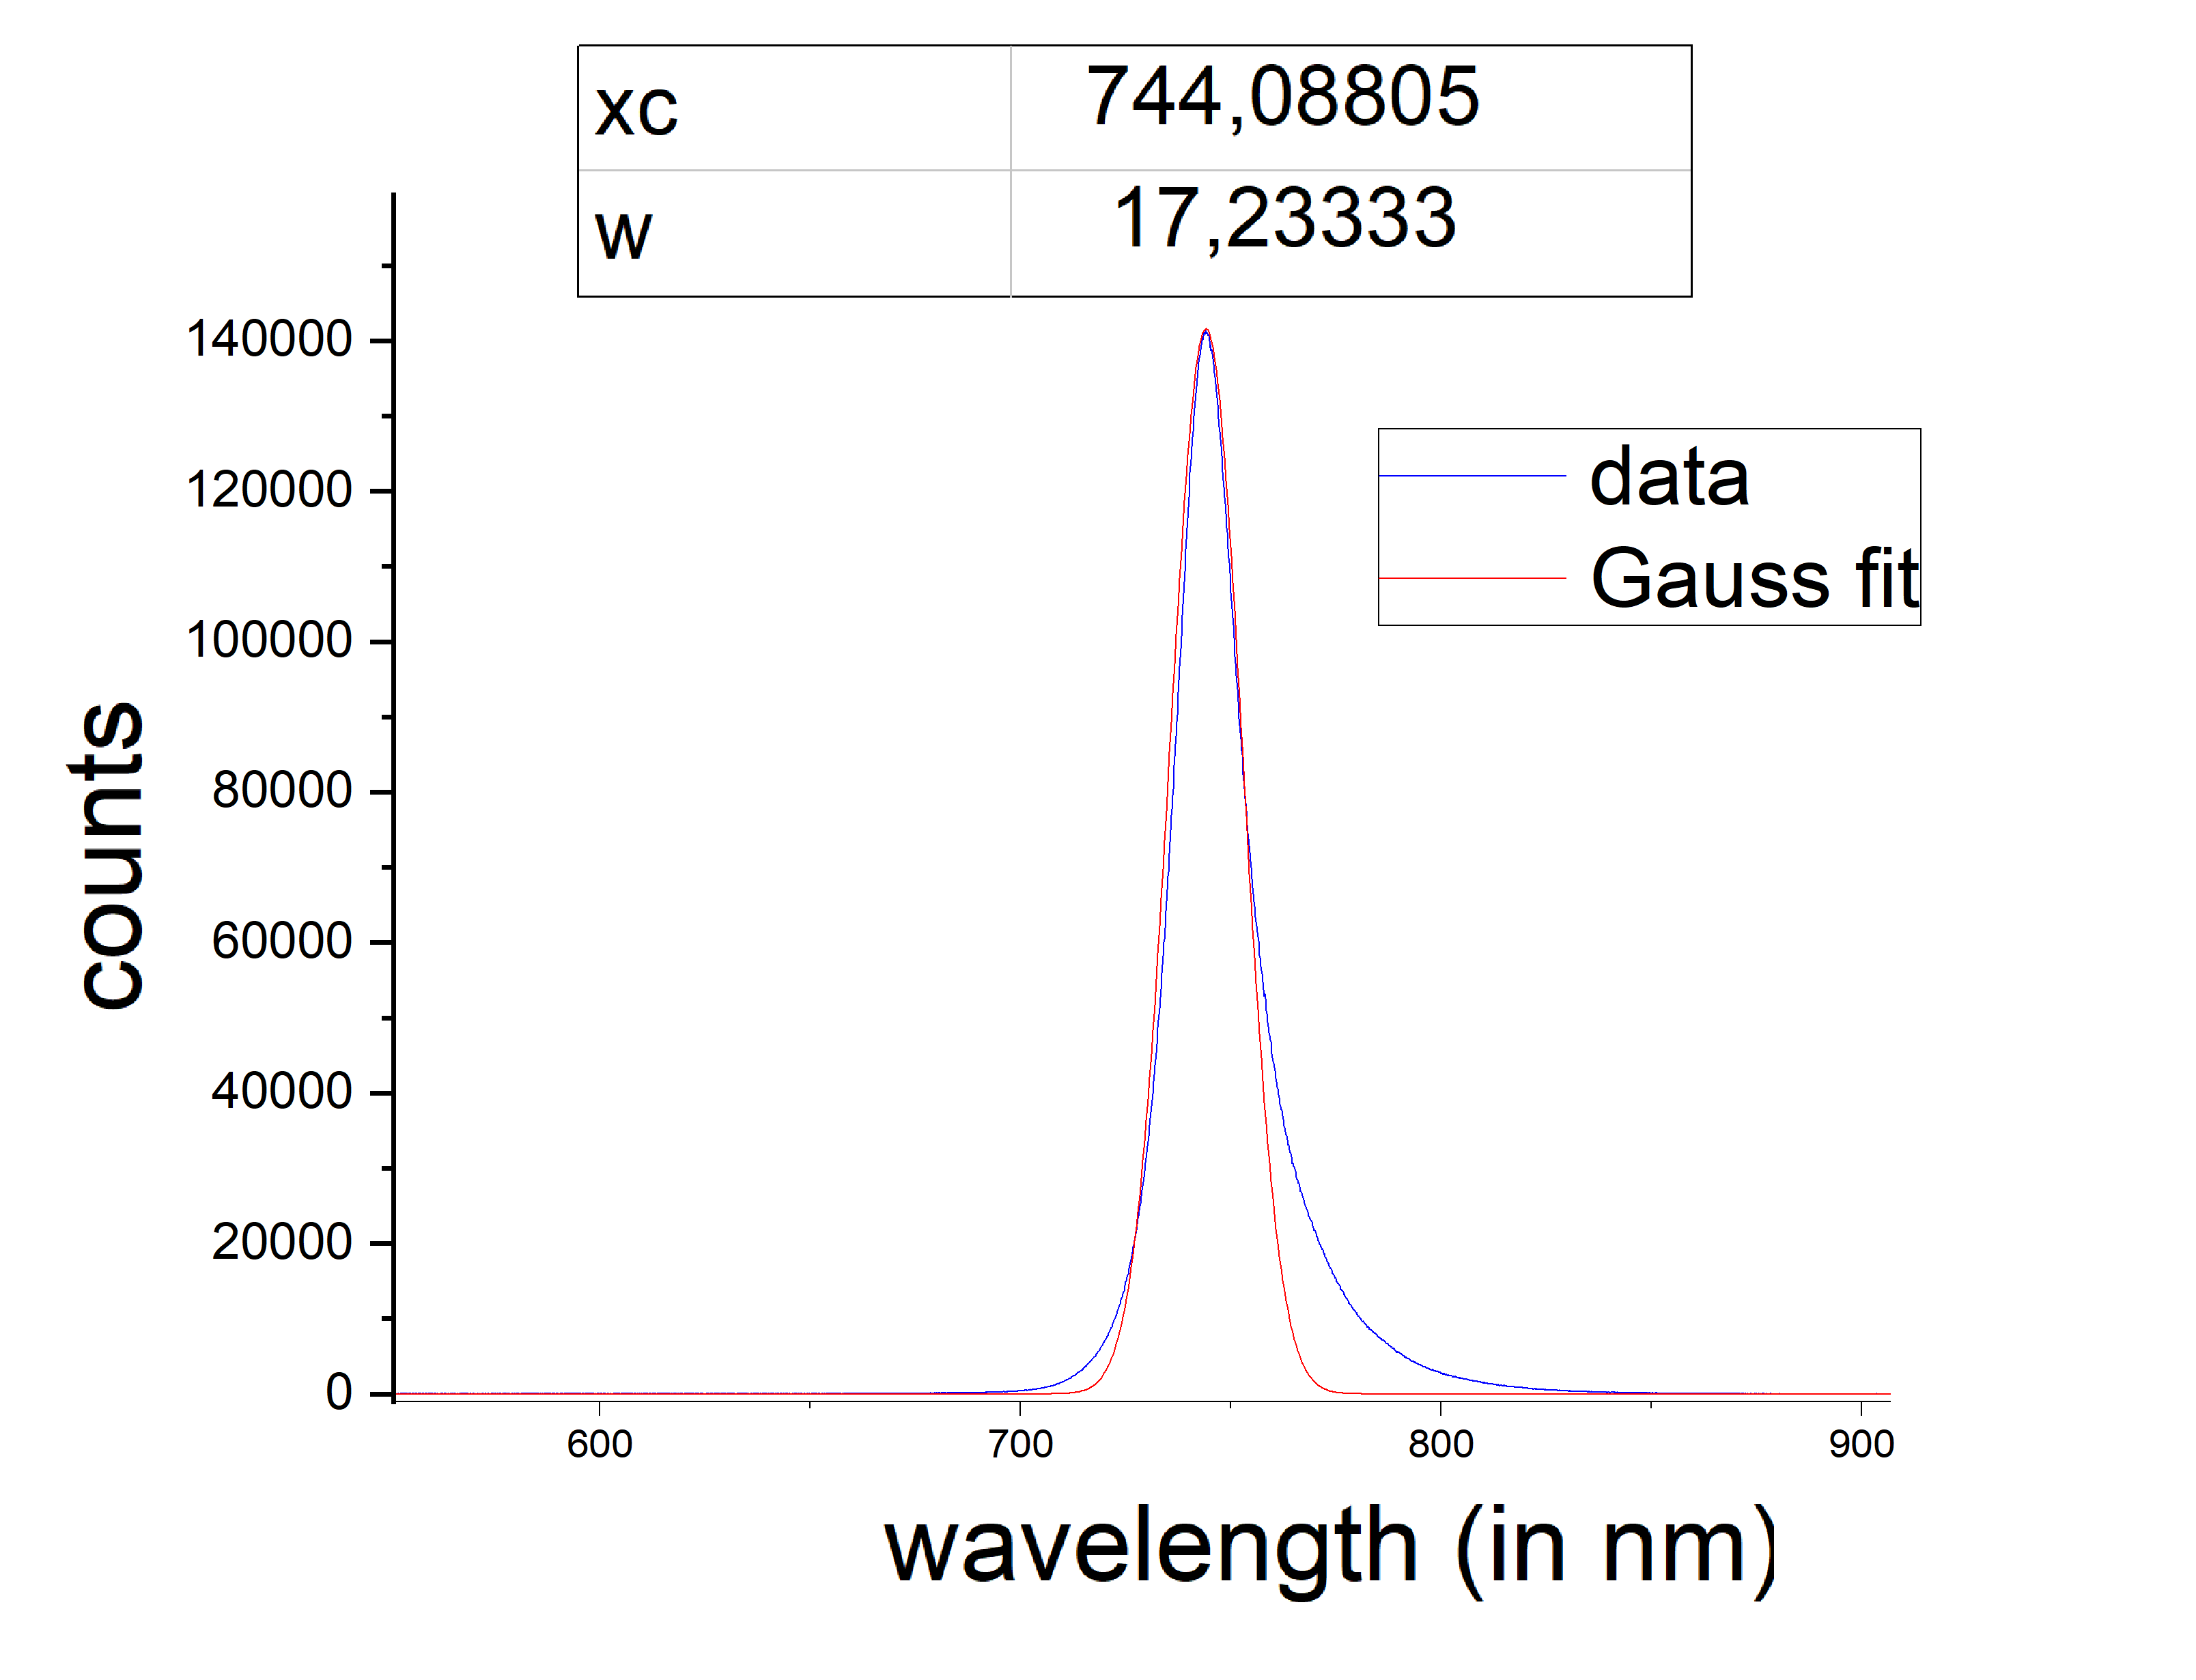
\includegraphics[width=\textwidth]{img/output_t1/spekt_m1-2-1}
        \caption{mat.1, spec. 2}
	      \label{fig_mono_spec2_1dspec}
    \end{subfigure}
    \begin{subfigure}{0.7\textwidth}
        \centering
        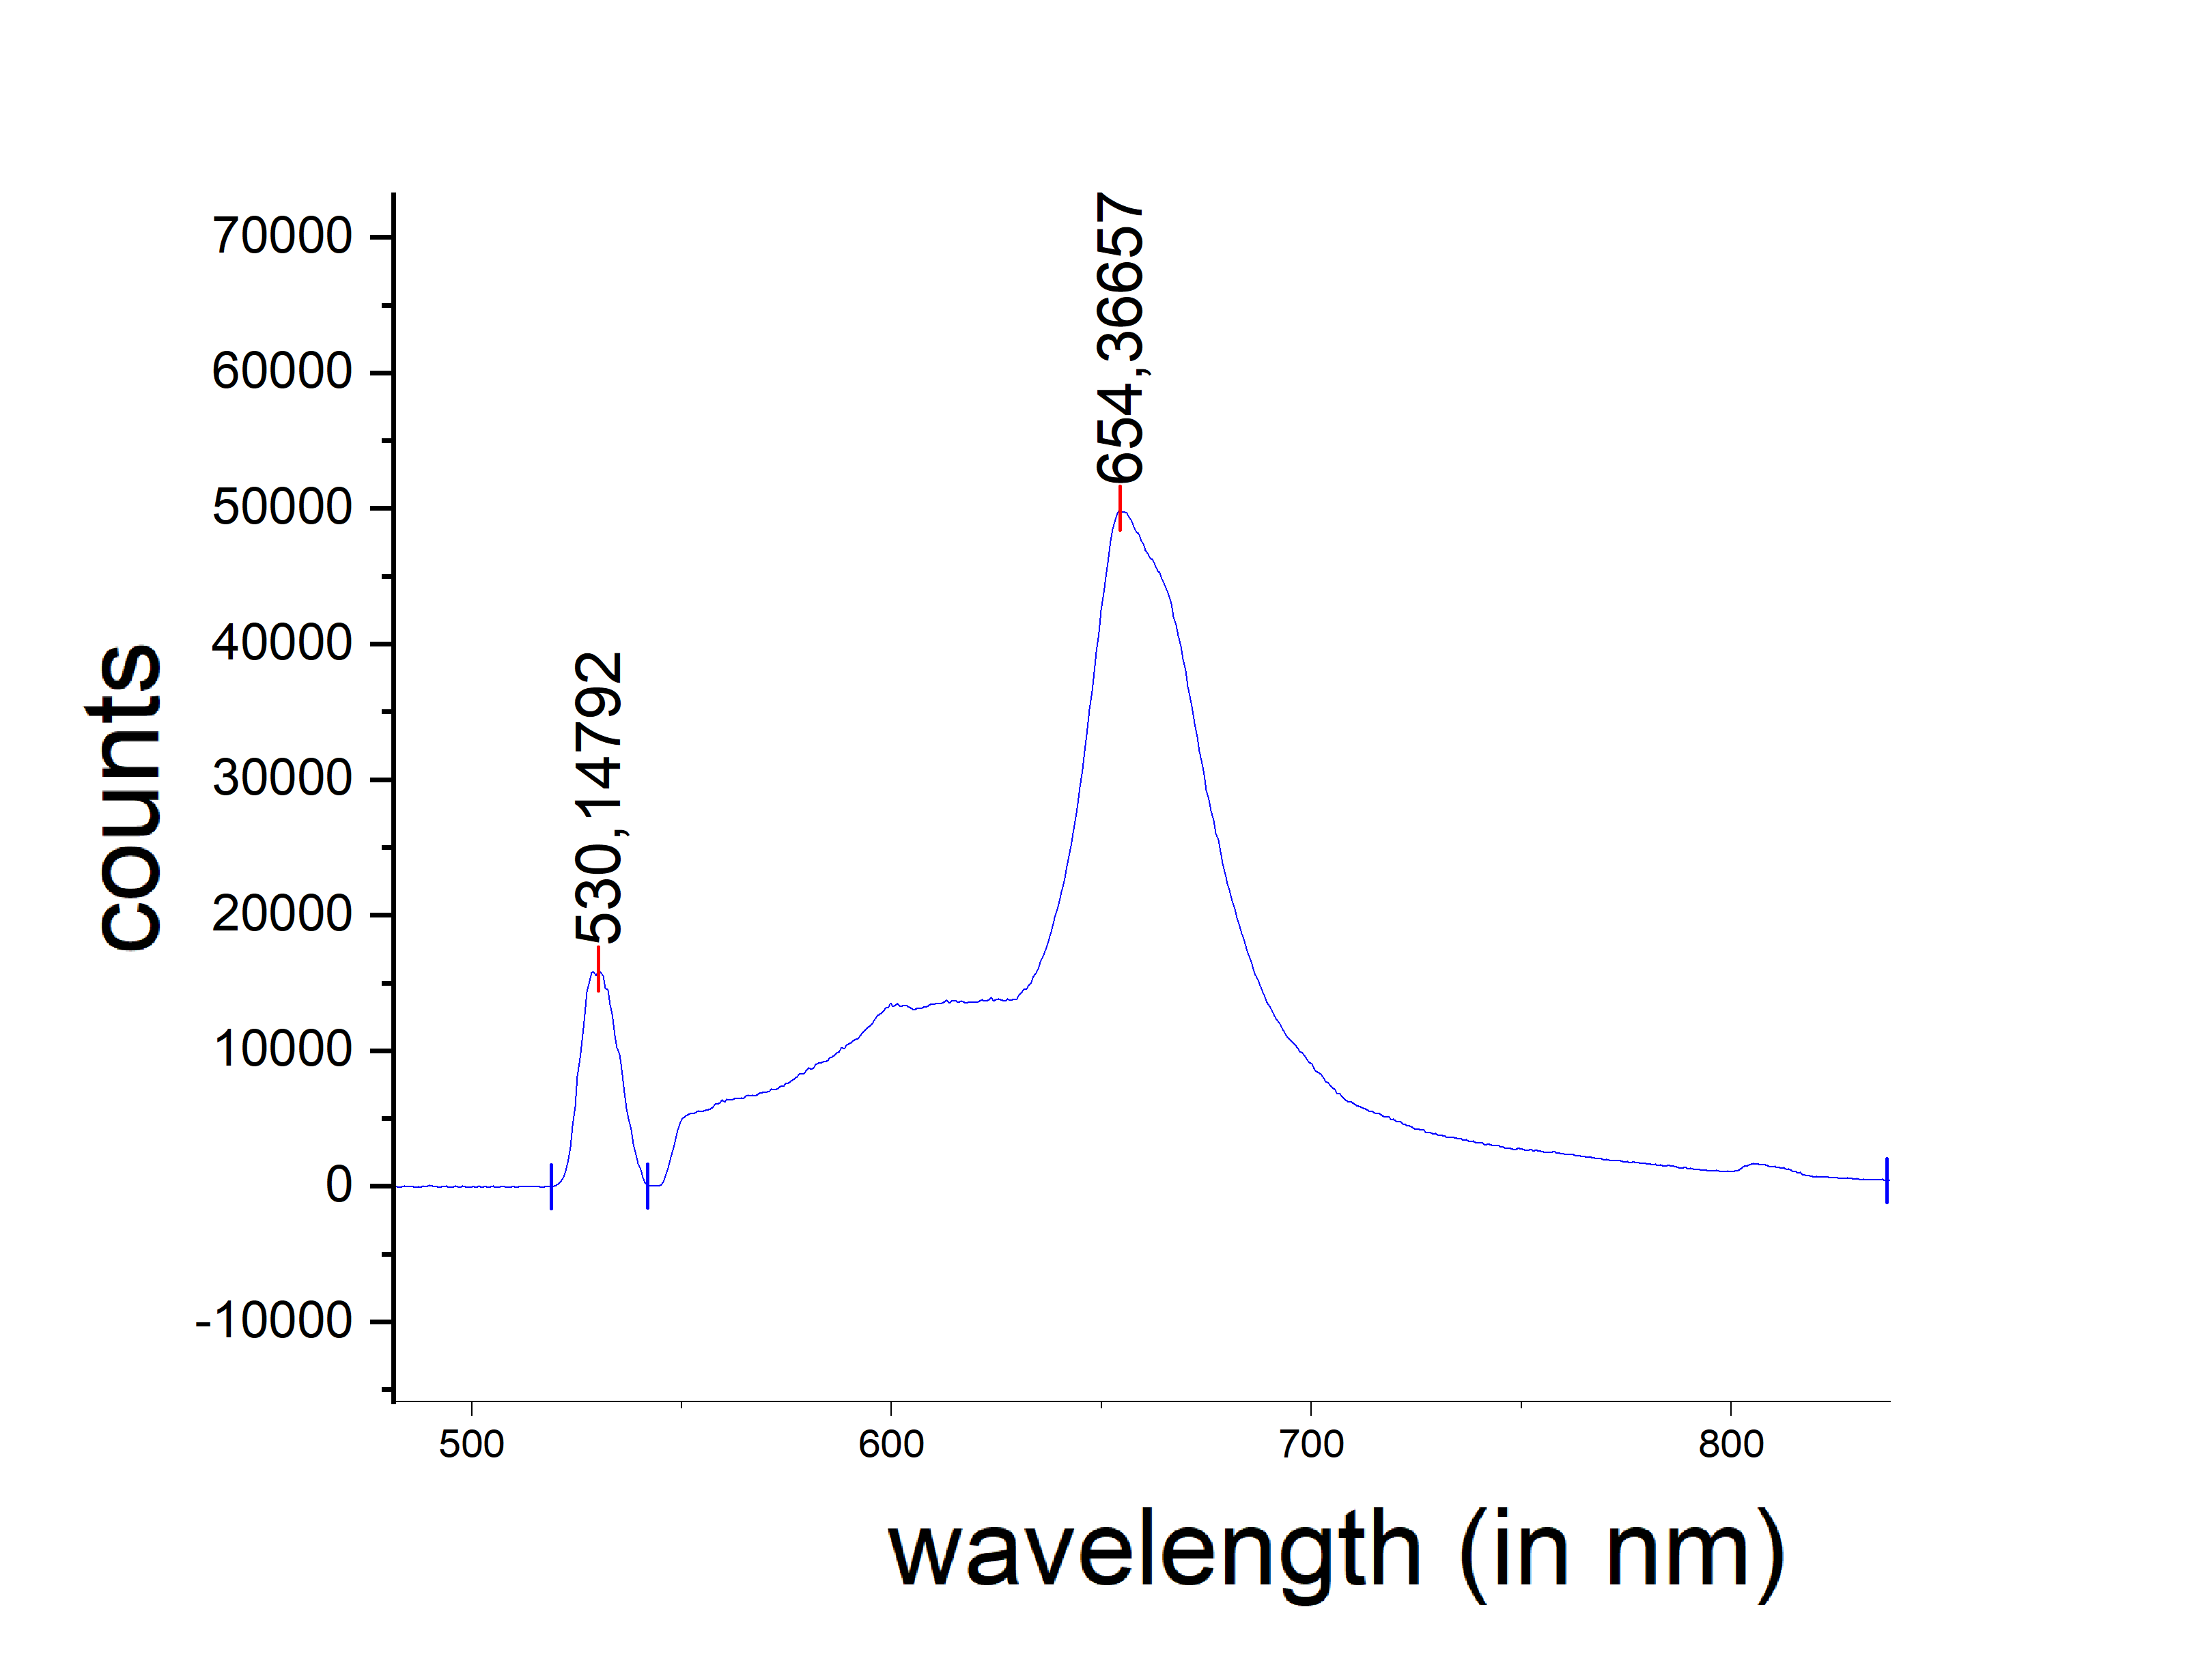
\includegraphics[width=\textwidth]{img/output_t1/spekt_m2}
        \caption{mat.2}
	      \label{fig_mono_spec3_1dspec}
    \end{subfigure}
    \caption{Measured Spectra for the two different materials. xc refers to the position of the peak and w is the FWHM.}
	\label{fig_mono_1dspectra} %mat2 -> 3
\end{figure}

From the spectra the peak positions can be used to assign the materials to specific TMDCs.
The measured peaks for material 1 are at \SI{746,5\pm 7,2}{nm} and \SI{744,1 \pm 7,2} for specimen 1 and 2, respectively, which may correspond to MoSe$_2$, monolayers of which emit at \SI{790}{nm}. \cite{Tonndorf2013}.
The difference may be due to not having measured a monolayer or change in the bandgap due to interaction with the substrate.
The measured peaks for material 2 lie at \SI{530,1 \pm 4,3}{nm} (A exciton) and \SI{654,4 \pm 6,8} (B exciton), allowing it to be assigned to monolayer WSe$_2$ with reasonable certainty.
The uncertainties are taken from the full width at half maximum (FWHM) according to $\sigma = \mathrm{FWHM}/(2\sqrt{2 \ln 2})$.
